\chapter{Introduction}
% ------------------------

\section{Aim and Background}
The aim of this project was to design an automated chip tester for the University
of Southampton Superchip, also known as D2. Undergraduates at the School of Electronics
and Computer Science participate every year in a project in which they
design a part of a digital chip. Figure \ref{fig:chip_overview} shows an overview
of the final chip, which includes up to 16 individual designs.
\begin{figure}[h!]
\centering
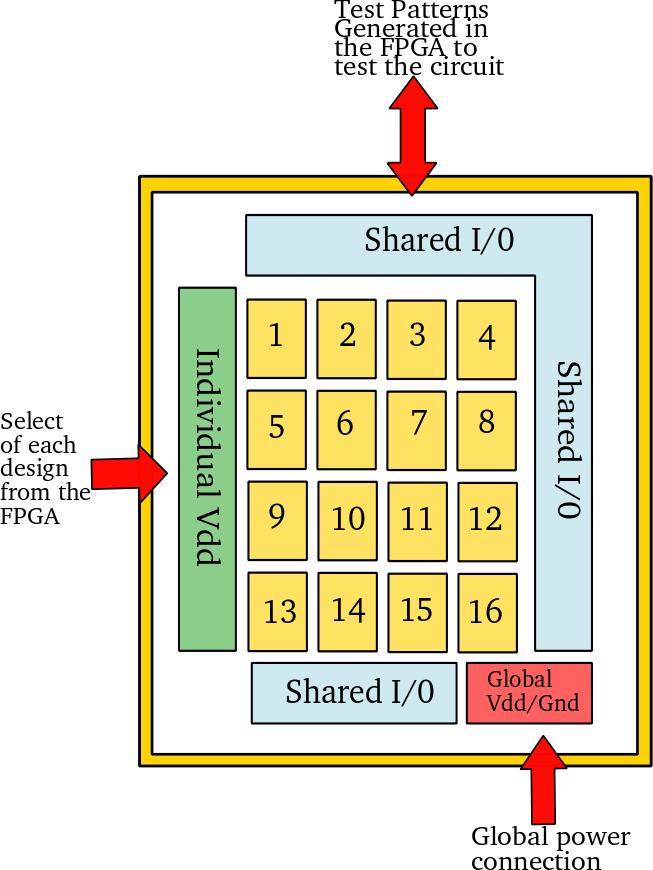
\includegraphics[scale=0.35]{Chip.png}
\caption{Overview of the Superchip (D2)}
\label{fig:chip_overview}
\end{figure}

All individual designs share the same 24 input and 24 output pins, but have separate power supplies.
As all of them share the same outputs, only one design can be active at any one time.
\\

Each of the 16 individual blocks on the chip is made up of smaller designs such as
adders, ring oscillators and other simple digital circuits. Every year one of the
smaller designs is an oscillator. As such, one of the requirements of the chip tester
is to measure the frequency of the on-chip oscillator.
\\

The chip tester was to be implemented using an Altera DE2-115 Development Board,
featuring an Altera Cyclone IV EP4CE115 FPGA.


\newpage
\section{DE2 Board Overview}
The DE2 board is an FPGA board designed by Terasic, based around an Altera
Cyclone IV FPGA. The following hardware relevant to this project is provided on
the DE2-115 board:

\begin{itemize}
 \item Altera Cyclone® IV EP4CE115 FPGA device
 \item USB Blaster (on board) for programming; both JTAG and Active Serial (AS) programming modes are supported
 \item 2MB SRAM (organized as 1M x 16 bits)
 \item 128MB SDRAM
 \item 8MB CFI Flash memory
 \item SD Card socket
 \item 50MHz oscillator
 \item 2 Gigabit Ethernet PHY with RJ45 connectors
 \item RS-232 transceiver and 9-pin connector
 \item One 40-pin Expansion Header with diode protection
 \item One High Speed Mezzanine Card (HSMC) connector
 \item 16x2 Character LCD display
\end{itemize}




\section{System Overview}

The Superchip tester designed within this project aims to provide a functional and user friendly testbench for the University of Southampton Superchips. To provide the required functionality, with a user-friendly interface and stable operation, the designed system can be considered into the following parts:

\begin{itemize}
 \item the main FPGA board (Altera DE2),
 \item the DUT board (Superchip),
 \item the secondary virtual design board (with programmable FPGA),
 \item the database server (also providing backend software and interface).
\end{itemize}

A graphical illustration of the overview of the system can be seen in figure \ref{fig:intro_sys_overview}.

\begin{figure}[h!]
\centering
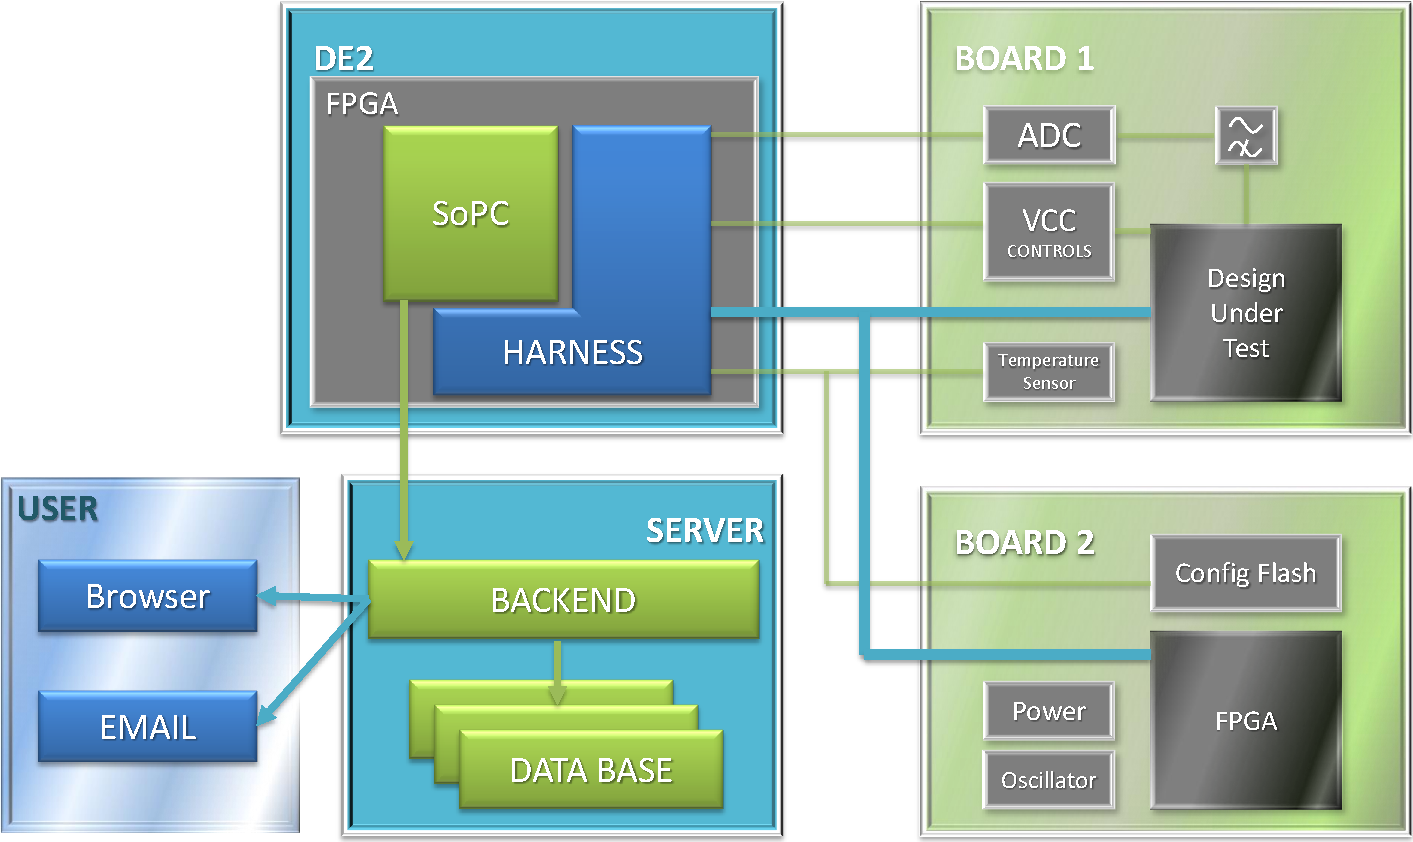
\includegraphics[width=0.9\textwidth]{sys_overview}
\caption{Overview of the ChipTester system designed for the ELEC6027 VLSI Group Design Project, Team I.}
\label{fig:intro_sys_overview}
\end{figure}

The DE2 main board hosts the SoPC core that provides the main functionality of the designed system and the harness to the device under test. The SoPC implements the chip testing functionality that is the main function of the project, implementing vector testing for the digital part of the DUT as well as frequency measurement of the oscillator on the DUT.

The two external boards are connected to the FPGA and are tested in the same manner for correct function. The primary DUT board hosts the physical Superchip to be tested and monitored, while the secondary FPGA board contains a re-programmable soft implementation of the design on the board FPGA, to provide inspection of the pre-fabrication behaviour of the design. This way, both the design itself, as well as the physical implementation can be tested more thoroughly.

The main DE2 board communicates with a backend server that holds a results database. The database is updated from the FPGA with test results, and also provides the user with the option to upload their digital designs to be transferred to the secondary board \hl{right?}. The server also provides an interface to the user, displaying the results of the database and allowing its management, and also sending e-mails with the test results.










